\documentclass[11pt]{article}
\usepackage[margin=1in]{geometry}
\usepackage{booktabs,amsmath,amssymb,xcolor,graphicx}
\usepackage{hyperref}\hypersetup{colorlinks=true,linkcolor=blue!50!black,urlcolor=blue!50!black}

\title{\textbf{Toy-world RL examples}\\[2pt]
\large fast architecture sanity --- renders, plots, and policy ablations}
\author{Aiko (Claude Code), for Dr.\ Cs.\ Hajdu (with Galambos \& Kati)}\date{2026-06-29 (JST)}

\begin{document}\maketitle

\begin{abstract}
\noindent Every RL env in the repo is MuJoCo (minutes-to-hours/verdict). This is a \textbf{physics-free toy
suite} that exercises the \emph{real} policy backbones (\texttt{mlp} / \texttt{hsikan} / \texttt{sa\_hsikan} /
\texttt{mixture}, \texttt{cr} vs \texttt{cr\_cheby}) across every RL regime in \textbf{seconds}: a 1-step
\textbf{bandit}, multi-step \textbf{grid}/\textbf{hex} navigation, a 2-agent \textbf{collaborative} task, and two
\textbf{mechanism probes} (holonomy, spike-rotor). The headline: off-holonomy everything ties (use the fast
SA-HSiKAN); the one place structure is load-bearing --- cycle holonomy --- is read \emph{only} by the rotor
(multiplicative transport), not by additive message-passing. That explains the standing HSiKAN-ties-MLP record.
\end{abstract}

\section{The worlds}
\begin{center}\small
\begin{tabular}{llll}
\toprule
world & module & regime & tests \\
\midrule
k-bandit & \texttt{sanity\_rl} & 1-step, signed ring & accuracy + B=1 deploy latency \\
grid / hex & \texttt{sanity\_worlds.LatticeNav} & multi-step, 4-/6-neighbour & credit assignment (hex = grid-cell substrate) \\
collaborative & \texttt{sanity\_worlds.CollabBandit} & 2-agent (CTDE) & coordination ($a_A+a_B$ matches a target) \\
holonomy / spike & \texttt{holonomy\_probe} / \texttt{spike\_probe} & supervised probes & is cycle holonomy load-bearing? \\
\bottomrule
\end{tabular}
\end{center}

\section{Renders}
The agent navigating the grid and hex worlds to its goal (GIFs delivered alongside; final frames below). The
policy reads per-vertex features over the lattice hypergraph and steers a continuous point to the goal landmark
over a 10-step horizon. Partial reach at this (seconds-long) budget --- the point is the loop runs end-to-end.

\begin{figure}[h]\centering
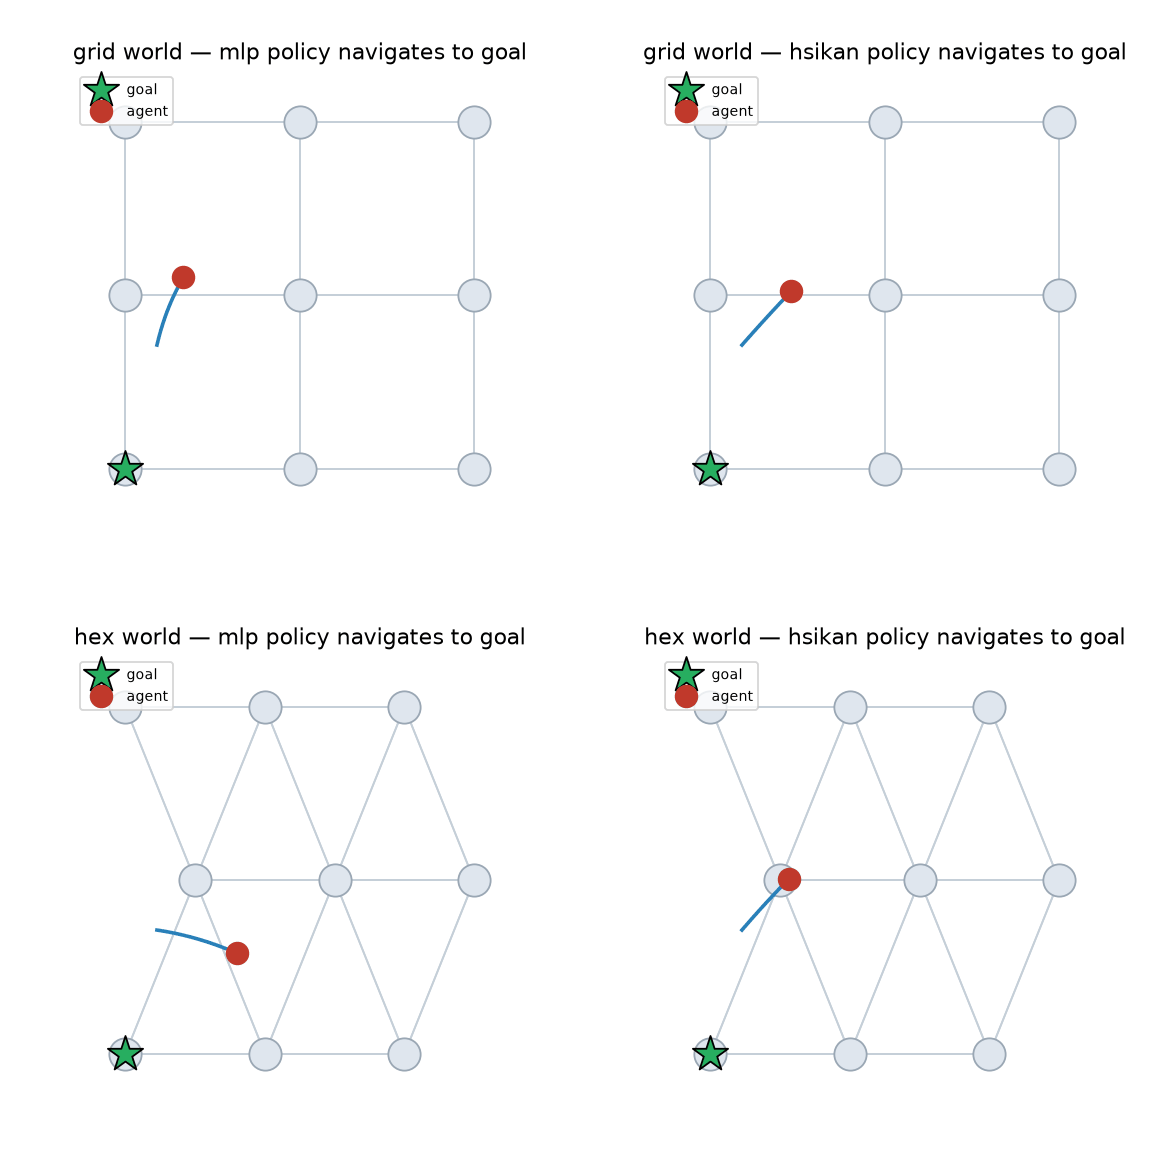
\includegraphics[width=0.62\textwidth]{figures/toy_worlds/nav_trajectories.png}
\caption{Trajectories (blue path, red agent, green star = goal) on the grid (top) and hex (bottom) lattices, for
the MLP (left) and HSiKAN (right) policies. Animated GIFs: \texttt{reports/figures/toy\_worlds/\{grid,hex\}\_nav\_*.gif}.}
\end{figure}

\section{Policy ablations (measured)}
\begin{figure}[h]\centering
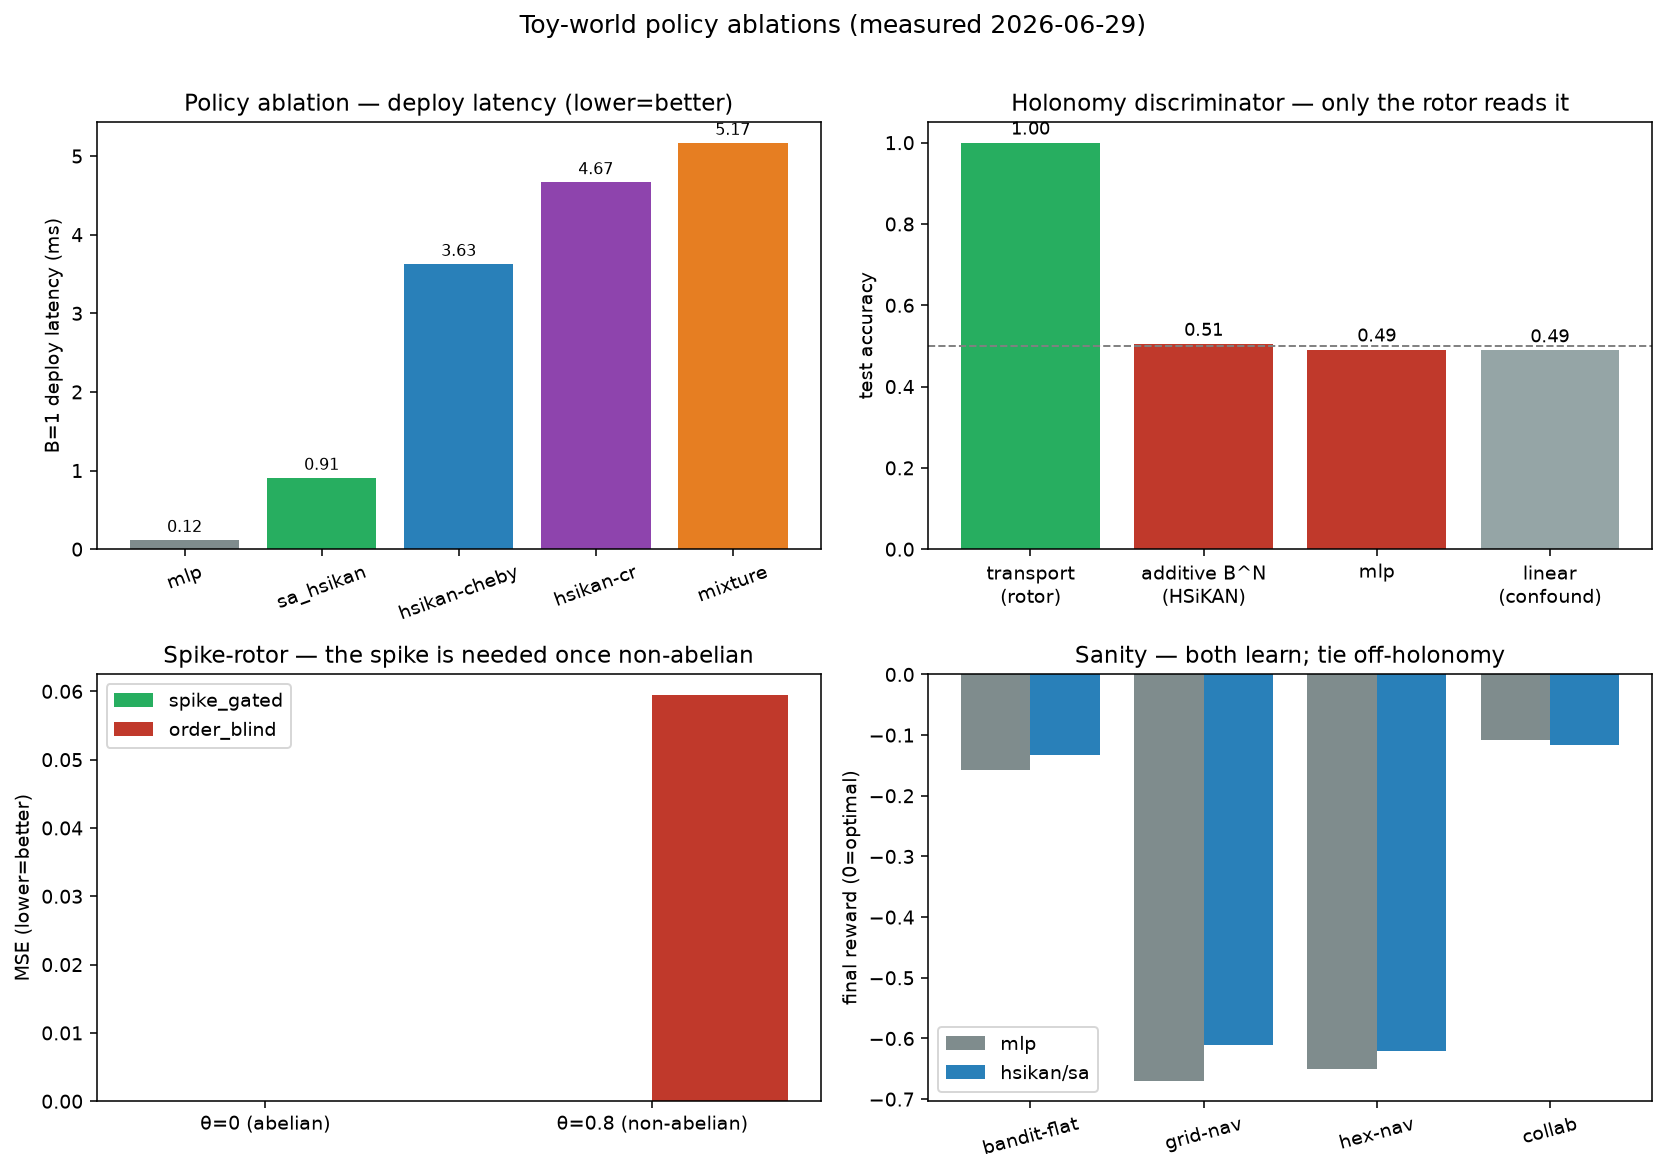
\includegraphics[width=\textwidth]{figures/toy_worlds/ablations.png}
\caption{Four ablations. \textbf{(A)} deploy latency --- SA-HSiKAN's B$^L$ collapse and the CR-Chebyshev deploy
path. \textbf{(B)} the holonomy discriminator. \textbf{(C)} spike-rotor. \textbf{(D)} sanity rewards.}
\end{figure}

\paragraph{(A) Deploy latency (B=1, the launch-bound regime).} SA-HSiKAN \textbf{0.91\,ms} (5$\times$ faster than
vanilla HSiKAN 4.67\,ms, 10$\times$ fewer params: 775 vs 8071); \texttt{cr\_cheby} deploy path 3.63\,ms
(\,$\sim$22\% faster than \texttt{cr}, same params, better reward). The recent perf work, visible in seconds.

\paragraph{(B) Holonomy --- the decisive discriminator (ring-16, 3 seeds).}
\begin{center}\small
\begin{tabular}{lcccc}
\toprule
arm & transport (rotor) & additive B$^N$ (=HSiKAN) & mlp & linear (confound) \\
\midrule
test acc & \textcolor{green!55!black}{\textbf{1.00}} & 0.50 & 0.50 & 0.49 \\
\bottomrule
\end{tabular}
\end{center}
The label is a clean Z$_2$ cycle holonomy (product of edge signs); the linear probe at chance proves there is no
local cue. \textbf{Holonomy is \emph{multiplicative} (parallel transport): the rotor reads it exactly; the
additive signed-walk B$^N$ --- HSiKAN's own mechanism --- is at chance, like the MLP.} This is the cleanest
explanation of why HSiKAN ties MLP: additive aggregation is not a holonomy reader.

\paragraph{(C) Spike-rotor.} On a non-abelian SO(3) connection ($\theta{=}0.8$): \texttt{spike\_gated} MSE 0.0 vs.\
\texttt{order\_blind} 0.059 --- the spike is needed to select the time-ordered walk. At $\theta{=}0$ (abelian) both
are exact (order is irrelevant). So the rotor reads abelian holonomy; the spike handles the non-abelian order.

\paragraph{(D) Sanity.} Bandit (flat), grid/hex nav, collab: every backbone learns (a broken one would fail here
in seconds). Off-holonomy, HSiKAN $\approx$ MLP --- structure is not load-bearing on these linear/acyclic tasks.

\section{Reading}
The toy suite turns hour-long architecture verdicts into seconds and pins down \emph{where} the structural power
lives: \textbf{the rotor (multiplicative transport) is load-bearing for cycle holonomy; everywhere else the
backbones tie, and the lever is the fast SA-HSiKAN / CR-Chebyshev path.} The collaborative regime trains and
coordinates (the fast analog of the Galambos delivery). \textbf{Next:} a rotor-equipped \emph{control} backbone on
a scenario with genuine cyclic structure (gait/contact cycles, closed kinematic loops) --- to convert ``the rotor
reads holonomy'' from a probe into a control result. Code: \texttt{hymeko\_rl/\{sanity\_rl,sanity\_worlds,
holonomy\_probe,spike\_probe\}.py}; 12 tests, ruff+mypy clean.
\end{document}
